\subsection{The shipped model and its in-browser runtime}\label{sec:shipped}

\ifWinIsDistillTwo
The shipped model is \emph{PhotonDistill2}, the locked winner of round 3 and the second generation of PhotonDistill. It is one trained student network. At inference it runs alone: no teacher, no gate and no chain.

\begin{figure}[t]
\centering
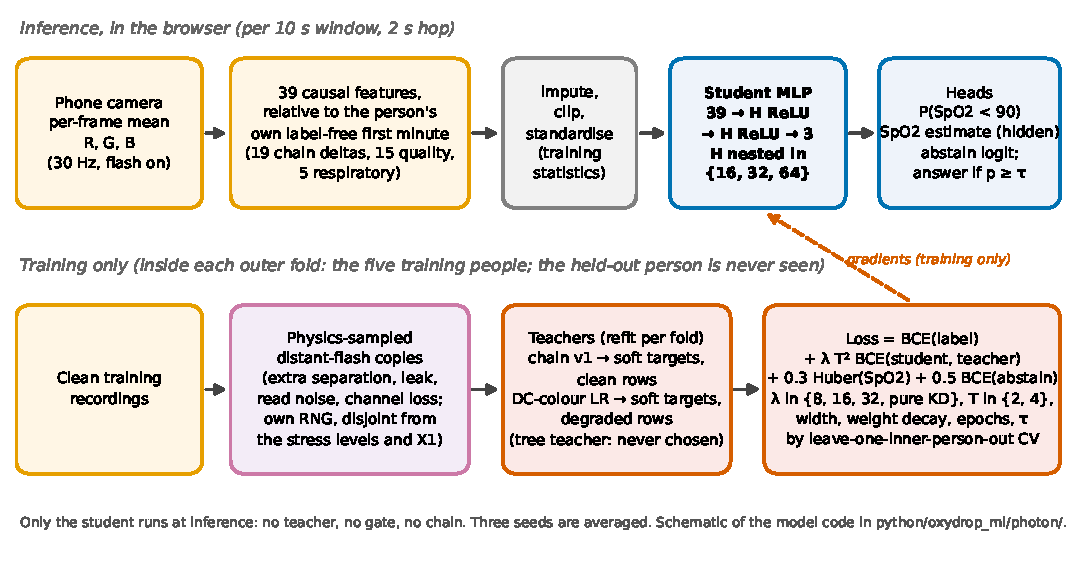
\includegraphics[width=0.95\linewidth]{figures/fig_arch.pdf}
\caption{PhotonDistill2. Top: inference in the browser. Bottom: training inside each fold. The teachers and the degraded copies exist only during training.}\label{fig:arch}
\end{figure}

\paragraph{Input.} Every 2~s the app computes 39 causal features of the last 10~s of per-frame mean R, G and B, each relative to the person's own label-free first minute: 19 chain deltas (heart-rate rise, ratio-of-ratios, pulse shape, DC colour), 15 signal-quality features and 5 respiratory features. The front end is the one of PhotonDistill. Imputation values, clipping bounds and standardisation come from the training people of the fold.

\paragraph{Network.} A multilayer perceptron $39\to H\to H\to3$ with ReLU activations. The hidden width $H\in\{16,32,64\}$ is chosen by nested cross-validation (2,435 parameters per student at $H=32$, 6,915 at $H=64$); the three deployed students have $H=32,32,64$ and are averaged. The three heads output the hypoxia logit (the score, $P(\spo{}<90\%)$), an \spo{} estimate in standardised units that the app never shows, and an abstain logit that predicts whether the hypoxia head is right. The model answers when the abstain probability reaches a threshold $\tau$ chosen on inner out-of-fold windows (answered accuracy and balanced accuracy at least 0.90).

\paragraph{Training inside each outer fold.} Two teachers are refit on the fold's five training people: the chain gives soft targets on clean windows, and a DC-colour logistic regression (three baseline-relative ln DC values) gives soft targets on physics-sampled distant-flash copies of the training recordings. A second teacher family that averages each of these with a gradient-boosted tree model was also in the search and was never chosen. The augmentation prior draws the extra separation, light leak, read noise and channel loss from declared ranges (four copies per training recording) from an independent random stream whose (level, seed) pairs are disjoint from the stress levels, and never samples X1. The loss is
\begin{equation}
\begin{split}
\mathcal L={}&\mathrm{BCE}(y,z)+\lambda_{\mathrm{kd}}T^2\,\mathrm{BCE}\big(\sigma(z/T),\,p_{\mathrm{teacher}}^{(T)}\big)\\
&+0.3\,\mathrm{Huber}(\widehat{\mathrm{SpO}}_2)+0.5\,\mathrm{BCE}\big(a,\mathbf{1}[\text{hypoxia head correct}]\big),
\end{split}
\end{equation}
with class balancing, clean windows weighted 1 and degraded windows 0.25, trained with Adam \citep{kingma2015adam} (learning rate $3\times10^{-3}$, batch 512). Pure distillation drops the label term. Selection is two-stage and nested, by leave-one-inner-person-out cross-validation on the criterion $0.5\,\mathrm{TM}(\text{clean})+0.5\,\mathrm{mean\,TM}(\text{degraded copies})$: first the teacher family, $\lambda_{\mathrm{kd}}\in\{8,16,32,\text{pure}\}$, $T\in\{2,4\}$ and epochs $\{15,30\}$ at width 32; then the width and weight decay $\{10^{-4},10^{-2}\}$ for the stage-one winner. Over the 18 seed folds, $\lambda_{\mathrm{kd}}=16$ was chosen 7 times and 32 nine times, $T=2$ 11 times and $T=4$ 7 times, width 32 ten times and 64 seven times, and 30 epochs 15 times (\texttt{results/photon/distill2\_log.md}). The grid edge that PhotonDistill hit (8 in all 18 folds) is now inside the grid. The planned PhotonTwin physics teacher and OxySeq or OxyTrack teachers were not used (the saved outputs of the latter two are leave-one-person-out predictions, so using them as teachers would leak).

\paragraph{Deployment.} The deployed weights are three students refit on all six people with the modal nested recipe of each seed ($\lambda_{\mathrm{kd}}=16,32,32$; $T=2,2,4$; $H=32,32,64$; weight decay $10^{-4}$; 30 epochs; mean $\tau=0.916$). The deployed model has therefore seen every Hoffman person, and the reported numbers are those of the leave-one-person-out fold models, not of the deployed files.

\paragraph{In-browser runtime.} The feature extractor is ported to JavaScript (\texttt{app/js/distill\_\allowbreak features.js}) and agrees with the Python extractor to $10^{-12}$ on fixture recordings. A small network runtime (\texttt{app/js/nn\_\allowbreak runtime.js}) executes plain operations (linear, 1D convolution, GRU, layer norm or folded batch norm, activations, pooling) from a JSON weight file in double precision and agrees with PyTorch to $4\times10^{-15}$ on its test network. The weights of PhotonDistill2 use the same file format as the round-2 engine, so the same app export script converts them without code changes, and the exported application forward pass reproduces the reference scores of two fixture windows to $2.4\times10^{-9}$. The app shows the model's output and abstention as they are, with fixed wording for the three states (Normal vs your baseline; Possible low oxygen, re-check with a pulse oximeter; Unsure, re-measure). Latency on phones was not measured for this paper. Nothing leaves the device.
\else
\TODO{The locked round-3 winner is \WinName{} (key \WinKey). Replace this subsection by its input, network, training, deployment and runtime description.}
\fi
